\documentclass[../../main.tex]{subfiles}

\begin{document}
    
    \section{Steganalysis}
    Steganalysis is the branch of study dedicated at analysing the methods and
    the vectors used to transmit an hidden message in order to retrieve such
    message whenever it is present. Usually we call steganalysis successfull when it is capable of detecting the presence of a \emph{stego message}
    Unlike cryptanalysis where the message may even be apparent but encrypted,
    in steganalysis the study of the message starts from a suspect.
    \subsection{Methods}
    Hereinafter we will present the methods used in steganalysis in
    order to obtain the secret message. The following image illustrates all of
    them. Here we simply want to introduce them in a rigorous way, but they will
    be treated in the specific cases when dealing with the cover types.

    \begin{figure}[h]
        \centering
        \caption{Steganalysis techniques}
        \vstretch{0.8}{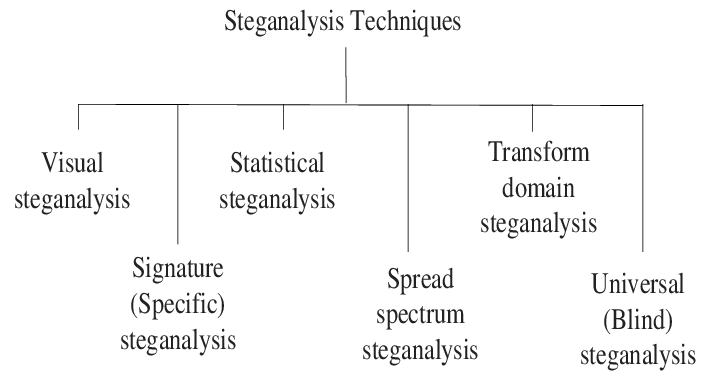
\includegraphics[scale=0.4]{classification_steganalysis.png}}
    \end{figure}


    \subsubsection{Statistical}
    Statistical steganalysis consists in using tools borrowed by Statistics in
    order to spot anaomalies in the cover message. These anomalies can be
    usually detected by searching in the data for patterns or by simply
    analysing some alteration of the modelled probability distribution of the
    data in the message. Often Neural Networks are involved in this type of
    steganalysis.

    \subsubsection{Visual}
    This is a very rudimental yet effective way of determining if a message was
    modified or not. This technique relies on the human eye and ita ability to
    spot anomalies in the format of a message which may pave the way for
    suspects.
    
    \subsubsection{Spread Spectrum}
    This is a technique borrowed by signal analysis which consists in treating
    the data on which we want to perform the analysis as a signal. Following
    this reasoning it is almost immediate to see that the stego message embedded
    into our data is nothing but noise in our signal. Finally the steganalysis
    is performed in this case just like any other type of signal analysis.

    \subsubsection{Signature}
    Signature is deeply correlated to the field of Watermarking. In many cases
    the data on which it was performed the steganography could have been signed.
    The insertion of the stego message inside the signed data may thus lead to
    the alteration in the digital dignature, making the message visible to the
    receiver.
    
    \subsubsection{Transform Domain}
    Even in this case the goal is to start from considering the data we are
    analysing as a signal. Then we try to transport this signal from a domain
    into another so that to make it invisible to the end user.
    
    \subsubsection{Universal}
    This is a type of analysis performed in a sort of bloind mode. In this case
    we don't care aboutt he medium through which the message was sent but we
    perform a series of operations(reading LSB for example) which have little to
    nothing to do with the message itself.

    \subsection{Cover types}
    In the following sections, we will treat several \emph{cover} in which
    steganography can be applied to hide data.
    In particular we will focus on some of the most common methods and how is
    possible to do a steganalysis process in order to detect and in some cases
    even retrieve the embedded information.
    Notice that different cover types requires completely different approaches
    due to intrinsic factors such as size, presence of redudant data,
    perceptibility of modification by a human or formats in which the bits of
    the cover are stored.
    
\end{document}